\documentclass[aps,prapplied,reprint,superscriptaddress,nofootinbib,floatfix]{revtex4-2}

\usepackage{amsmath,amssymb}
\usepackage[hidelinks]{hyperref}
\usepackage{tikz}
\usepackage{pgfplots}
\pgfplotsset{compat=1.18}
\usetikzlibrary{arrows.meta,positioning}

\newcommand{\code}[1]{\texttt{#1}}

\begin{document}

\title{NVision: A Sequential Monte Carlo Framework for Bayesian Experiment Design\\
in Nitrogen-Vacancy Center Magnetometry}

\author{NVision Project}
\affiliation{Simulation framework described herein; physical implementation not performed.}

\date{\today}

\begin{abstract}
Optically detected magnetic resonance (ODMR) of nitrogen-vacancy (N-V$^-$) centers in diamond is a leading
platform for nanoscale magnetometry, but conventional frequency-swept measurement wastes most of its budget
sampling far from resonance. Sequential Bayesian experiment design (SBED) instead chooses each measurement
to maximize expected information gain (EIG) about the resonance parameters \citep{dushenko2020sbed}. This
paper describes \emph{NVision}, which extends this idea with a Sequential Monte Carlo (SMC) particle belief
on a dimension-agnostic unit cube, scaling to Zeeman-split, hyperfine-split, and Voigt-broadened lineshapes
with up to seven parameters. An EIG-maximizing acquisition rule, a closed-form Cram\'er--Rao lower bound
(CRLB) per lineshape, and a multi-criterion stopping test jointly decide where to measure and when to stop.
We present the signal models, the inference/acquisition mathematics, the simulation-harness architecture,
and the evaluation metrics, all cross-checked against the reference implementation.
\end{abstract}

\maketitle

% =====================================================================
\section{Introduction}
% =====================================================================

Nitrogen-vacancy (N-V$^-$) centers are diamond point defects with a spin-1 ground state whose $m_s=\pm1$
sublevels Zeeman-split under an external field (Fig.~\ref{fig:nv-levels}); spin-dependent fluorescence makes
this splitting optically readable as dips in an ODMR spectrum
\citep{doherty2013nv,balasubramanian2008,maze2008}. This makes N-V$^-$ magnetometry a widely used nanoscale
and vector field-sensing tool \citep{schloss2018vector}.

Conventional ODMR sweeps frequency over a fixed grid, wasting most measurements far from resonance where
they barely change the fit uncertainty. \citet{dushenko2020sbed} showed that choosing each frequency to
maximize a posterior-based utility function instead — SBED — cuts the required measurements by more than an
order of magnitude, using a two-parameter (frequency, linewidth) grid posterior and the \code{OptBayesExpt}
library.

NVision generalizes this along three axes absent from that work and from an earlier internal HUJI course
attempt at the same problem \citep{giat2024projectbook} (Table~\ref{tab:novelty}; bold = new here).

\begin{table}[t]
\centering
\caption{What NVision introduces relative to the two prior attempts. Bold = new here; plain = inherited.}
\label{tab:novelty}
\small
\begin{ruledtabular}
\begin{tabular}{p{2.1cm}p{2.5cm}p{2.9cm}}
Aspect & Prior attempts & \textbf{This work} \\
\colrule
Posterior & \code{OptBayesExpt} grid, $\le2$--3 params & \textbf{$N$-particle SMC, unit cube, up to 7} \\
Signal models & Bare Lorentzian / one triplet & \textbf{4 lineshape families} (hyperfine, Zeeman, Voigt, saturation) \\
Stopping rule & Fixed tolerance / iteration count & \textbf{Closed-form per-lineshape CRLB budget} \\
\end{tabular}
\end{ruledtabular}
\end{table}

The particle-based unit-cube belief (Section~\ref{sec:smc}) is what makes the richer, multi-parameter
lineshapes of Section~\ref{sec:physics} tractable in place of the grid both prior attempts share; the
CRLB-derived stopping rule (Sections~\ref{sec:crlb}--\ref{sec:convergence}) is the paper's most concrete
methodological contribution, replacing a hand-tuned tolerance with one grounded in the measurement's own
information content. The EIG-maximization principle itself is \citeauthor{dushenko2020sbed}'s
\citep{dushenko2020sbed,chaloner1995bayesian}, and unlike that work — validated on real N-V$^-$ hardware —
NVision is simulation-only (Section~\ref{sec:discussion}).

Section~\ref{sec:physics} covers the physical models and simulation architecture; Sections
\ref{sec:smc}--\ref{sec:convergence} the inference/acquisition math; Section~\ref{sec:metrics} the evaluation
metrics; Section~\ref{sec:discussion} scope and limitations.

% =====================================================================
\section{Physical Model and Experiment Layout}
\label{sec:physics}
% =====================================================================

\subsection{N-V center structure and Zeeman splitting}

An external field $B$ along the N-V axis splits $m_s=\pm1$ symmetrically about the zero-field frequency
$f_B\approx2.87$~GHz by $\gamma_{\rm NV}B$ ($\gamma_{\rm NV}\approx28$~GHz/T), producing two Zeeman dips
(Fig.~\ref{fig:nv-levels}); each is further split into a $^{14}$N hyperfine triplet ($\approx2.16$~MHz) with
finite homogeneous and inhomogeneous linewidth. Section~\ref{sec:signal-models}'s lineshapes implement this
hierarchy as composable, independently toggleable variants.

\begin{figure}[t]
\centering
\resizebox{0.95\linewidth}{!}{%
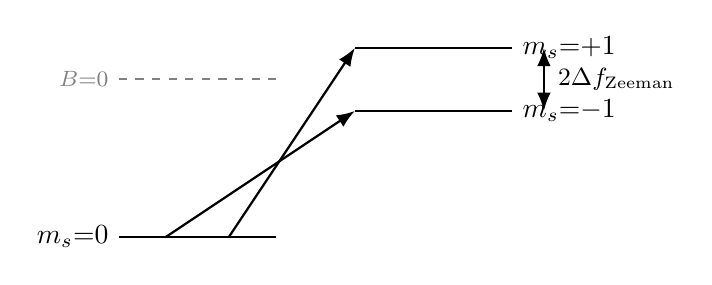
\begin{tikzpicture}[>=Latex, thick]
  \draw (0,0) -- (2,0);
  \node[left] at (0,0) {$m_s{=}0$};
  \draw[dashed,gray] (0,2) -- (2,2);
  \node[left,gray] at (0,2) {\footnotesize $B{=}0$};
  \draw (3,2.4) -- (5,2.4);
  \node[right] at (5,2.4) {$m_s{=}{+}1$};
  \draw (3,1.6) -- (5,1.6);
  \node[right] at (5,1.6) {$m_s{=}{-}1$};
  \draw[->] (0.6,0) -- (3,1.6);
  \draw[->] (1.4,0) -- (3,2.4);
  \draw[<->] (5.4,1.6) -- (5.4,2.4);
  \node[right] at (5.45,2.0) {\small $2\Delta f_{\rm Zeeman}$};
\end{tikzpicture}}
\caption{NV$^-$ ground-state spin triplet: field $B$ splits $m_s{=}\pm1$ symmetrically about
$f_B\approx2.87$~GHz by $\gamma_{\rm NV}B$; microwave transitions from $m_s{=}0$ (arrows) give the two
Zeeman-split ODMR dips.}
\label{fig:nv-levels}
\end{figure}

\subsection{Signal models}
\label{sec:signal-models}

All models are built around a single-Lorentzian-dip kernel
\begin{equation}
  L(x; f, \Omega) = \frac{\Omega^2}{\Omega^2 + (x-f)^2},
  \label{eq:lorentzian-kernel}
\end{equation}
unit height at $x=f$, HWHM $\Omega$ (FWHM $=2\Omega$).

\paragraph{Lorentzian triplet (\code{NVCenterLorentzianModel}).} With hyperfine splitting on,
\code{nv\_center\_lorentzian\_eval} uses a population-normalized reparameterization so the three dip weights
always sum to the total contrast $c$ (Fig.~\ref{fig:triplet-shape}):
\begin{widetext}
\begin{equation}
  p_{\rm sum} = \frac1{k_{\rm np}} + 1 + k_{\rm np}, \qquad
  p_0 = \frac{c}{p_{\rm sum}}, \quad
  p_L = \frac{c}{k_{\rm np}\,p_{\rm sum}}, \quad
  p_R = \frac{c\,k_{\rm np}}{p_{\rm sum}}, \qquad (p_L+p_0+p_R \equiv c),
  \label{eq:triplet-pop}
\end{equation}
\begin{equation}
  S(x) = 1 - \Big[p_L\, L(x; f_0 - \Delta f, \Omega) + p_0\, L(x; f_0, \Omega) + p_R\, L(x; f_0 + \Delta f, \Omega)\Big],
  \label{eq:triplet}
\end{equation}
\end{widetext}
\noindent $k_{\rm np}\in[1,5]$. Unlike Eq.~(1) of \citet{dushenko2020sbed}, where $k_{\rm np}$ scales two raw
amplitudes without renormalizing, $k_{\rm np}$ here only redistributes $c$ between dips. With hyperfine
splitting off, $\Delta f$ is fixed to 2.16~MHz and $k_{\rm np}=1$ (equal-weight triplet): the code calls this
the ``single dip'' configuration, but Eq.~\eqref{eq:triplet} is still evaluated at nonzero splitting — only
the number of \emph{inferred} parameters drops (3 vs.\ 5 with hyperfine on), not the underlying triplet
structure, which visually blends into one dip only once $\Omega\gtrsim\Delta f$. With Zeeman splitting on,
each dip weight in Eq.~\eqref{eq:triplet-pop} is halved and the triplet duplicated at $f_0\mp\Delta
f_{\rm Zeeman}$ (up to six free parameters, two dip clusters).

\begin{figure}[t]
\centering
\begin{tikzpicture}
\begin{axis}[
  width=\linewidth, height=4.2cm,
  xlabel={$(x-f_0)/\Omega$}, ylabel={$S(x)$},
  ymin=0, ymax=1.05, xmin=-8, xmax=8,
  domain=-8:8, samples=300,
  axis lines=left, tick align=outside,
  label style={font=\small}, tick label style={font=\scriptsize},
]
\addplot[thick] {1 - (1/7)/(1+(x+4)^2) - (2/7)/(1+x^2) - (4/7)/(1+(x-4)^2)};
\end{axis}
\end{tikzpicture}
\caption{Lorentzian triplet, Eq.~\eqref{eq:triplet}, for $k_{\rm np}=2$, $\Delta f/\Omega=4$: weights
$p_L{=}c/7,p_0{=}2c/7,p_R{=}4c/7$ ($c{=}1$) sum exactly to $c$.}
\label{fig:triplet-shape}
\end{figure}

\paragraph{Pseudo-Voigt triplet (\code{NVCenterVoigtModel}).} Each dip is a two-width pseudo-Voigt profile
(\code{nv\_center\_pseudo\_voigt\_eval}), height-normalized as
\begin{equation}
  V(x) = \frac{e_{\rm lf}}{x^2+\gamma_{\rm hom}^2} + e_{\rm gf}\,\exp\!\left(-\frac{x^2}{2\sigma_{\rm inhom}^2}\right),
  \label{eq:pseudovoigt}
\end{equation}
with $\gamma_{\rm hom}=\tfrac12\ell_{\rm frac}\Gamma$, $\sigma_{\rm inhom}=\tfrac12(1-\ell_{\rm frac})\Gamma/\sqrt{2\ln2}$
splitting total FWHM $\Gamma$ by Lorentzian fraction $\ell_{\rm frac}\in[0,1]$, and $e_{\rm lf},e_{\rm gf}$
fixed via the Thompson--Cox--Hastings weight $\eta$ so $V(0)=1$ — algebraically the code's on-the-fly
normalization, pre-factored. This is not a true Voigt profile (no Faddeeva function), and $\eta$ is
calibrated for a shared FWHM rather than the split widths used here, so the true-Voigt approximation error is
uncontrolled.

Unlike the Lorentzian family, this triplet is \emph{not} population-normalized: \code{dip\_depth} $d$ sets
the right-dip depth directly, with center and left dips at $d/k_{\rm np}$ and $d/k_{\rm np}^2$,
\begin{widetext}
\begin{equation}
  S(x) = 1 - \left[\frac{d}{k_{\rm np}^2}\,V(x-f_0+\Delta f) + \frac{d}{k_{\rm np}}\,V(x-f_0) + d\,V(x-f_0-\Delta f)\right],
\end{equation}
\end{widetext}
\noindent so total contrast is not held fixed as $k_{\rm np}$ varies, unlike Eq.~\eqref{eq:triplet}. Population
normalization reappears only in the saturation-coupled model below, which always routes through the
Zeeman-population kernel ($\Delta f_{\rm Zeeman}{=}0$ when Zeeman splitting is off).

\paragraph{Saturation-coupled Voigt (\code{NVCenterSaturationVoigtModel}).} Linewidth and contrast are coupled
through one drive parameter $s$ (power relative to half-saturation), since both are set by the same
microwave field:
\begin{equation}
  \gamma_{\rm hom}(s) = \gamma_0 \sqrt{1+s}, \qquad
  C(s) = c_{\max}\frac{s}{1+s},
  \label{eq:saturation-coupling}
\end{equation}
with fixed zero-power HWHM $\gamma_0=150$~kHz and saturated contrast $c_{\max}$. The independent Gaussian
width $\sigma_{\rm inhom}$ is uncoupled to drive power. $(s,\sigma_{\rm inhom},c_{\max})$ re-parameterizes into
$(\Gamma,\ell_{\rm frac},c)$ of Eq.~\eqref{eq:pseudovoigt} before evaluation; $\sigma_{\rm inhom}\to0$ recovers
a pure Lorentzian exactly.

\subsection{Physical parameter ranges}

Table~\ref{tab:bounds} lists the physical bounds shared by the signal generator and the SMC prior, so the two
cannot drift apart.

\begin{table*}[t]
\centering
\caption{Representative physical parameter bounds (Lorentzian/Voigt family).}
\label{tab:bounds}
\begin{ruledtabular}
\begin{tabular}{llr}
Parameter & Symbol & Range \\
\colrule
Center frequency domain & $f_0$ & $2.6$--$3.1$~GHz \\
Linewidth (HWHM) & $\Omega$ & $200$~kHz--$5.0$~MHz \\
Hyperfine splitting & $\Delta f$ & $2.0$--$8.5$~MHz \\
Nuclear-polarization asymmetry & $k_{\rm np}$ & $1.0$--$5.0$ \\
Zeeman half-separation & $\Delta f_{\rm Zeeman}$ & $0$--$100$~MHz ($\approx$ 0--3.6~mT) \\
Natural (zero-power) HWHM & $\gamma_0$ & $150$~kHz (fixed) \\
$^{14}$N hyperfine constant & --- & $2.16$~MHz (fixed, when not inferred) \\
Saturation parameter & $s$ & $0.02$--$30$ \\
\end{tabular}
\end{ruledtabular}
\end{table*}

\subsection{Simulation harness architecture}
\label{sec:architecture}

Each simulated experiment is a Generator$\times$Noise$\times$Locator task (Fig.~\ref{fig:architecture}): a
ground-truth signal (Section~\ref{sec:signal-models}), an additive Gaussian noise floor (this paper's scope;
Poisson and Rao-Blackwellized inverse-gamma models exist but are not covered), and an acquisition-and-stopping
strategy (uniform/Sobol baselines or a Bayesian locator). The Runner executes many tasks concurrently over
independent, seed-deterministic, resumable repeats, streaming results to an on-disk cache for large repeat
counts, and automatically runs a matched Sobol baseline for every Bayesian strategy under identical noise and
ground truth. Within a repeat, \code{next()}/\code{observe()}/\code{done()} iterate until the stopping
criteria of Section~\ref{sec:convergence} fire, recording the metrics of Section~\ref{sec:metrics}.

\begin{figure}[t]
\centering
\resizebox{\linewidth}{!}{%
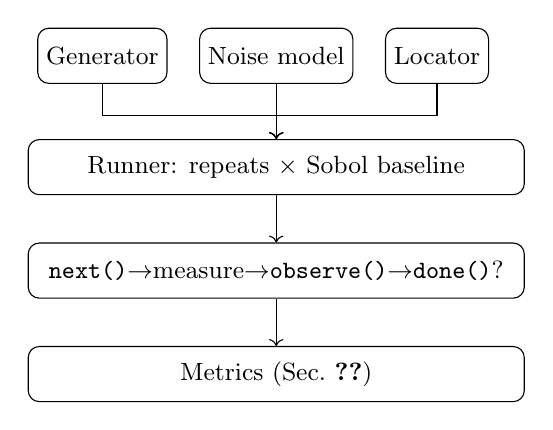
\begin{tikzpicture}[node distance=5mm, font=\small,
  box/.style={draw,rounded corners,align=center,minimum height=7mm,inner sep=3pt}]
  \node[box] (gen) {Generator};
  \node[box, right=4mm of gen] (noise) {Noise model};
  \node[box, right=4mm of noise] (loc) {Locator};
  \node[box, below=7mm of noise, minimum width=6.3cm] (runner) {Runner: repeats $\times$ Sobol baseline};
  \node[box, below=6mm of runner, minimum width=6.3cm] (loop) {\code{next()}$\to$measure$\to$\code{observe()}$\to$\code{done()}?};
  \node[box, below=6mm of loop, minimum width=6.3cm] (metrics) {Metrics (Sec.~\ref{sec:metrics})};
  \draw[->] (gen.south) -- ++(0,-4mm) -| (runner.north);
  \draw[->] (noise) -- (runner);
  \draw[->] (loc.south) -- ++(0,-4mm) -| (runner.north);
  \draw[->] (runner) -- (loop);
  \draw[->] (loop) -- (metrics);
\end{tikzpicture}}
\caption{Simulation harness: a Generator$\times$Noise$\times$Locator task runs under the Runner across
independent repeats (Sec.~\ref{sec:architecture}), iterating until the stopping criteria of
Sec.~\ref{sec:convergence} fire.}
\label{fig:architecture}
\end{figure}

% =====================================================================
\section{Sequential Monte Carlo Belief}
\label{sec:smc}
% =====================================================================

The posterior over $d$ free parameters $\boldsymbol\theta$ is $N$ weighted particles
$\{(\boldsymbol\theta_i,w_i)\}_{i=1}^N$, scaling to $d>2$ without the grid's exponential memory blow-up — the
mechanism enabling Section~\ref{sec:signal-models}'s six-parameter models.

\subsection{Unit-cube / physical coordinate separation}
\label{sec:unitcube}

All particle arithmetic happens on a dimension-agnostic unit cube $[0,1]^d$; each parameter $j$ maps to its
physical bound $[l_j,h_j]$ via a fixed affine rescale map,
\begin{equation}
  \theta_j^{\rm phys} = l_j + u_j\,(h_j - l_j), \qquad
  \sigma_j^{\rm phys} = \sigma_j^{u}\,(h_j - l_j),
  \label{eq:rescale}
\end{equation}
owned exclusively by the belief and fixed for a run's lifetime. This is kept strictly separate from the
\emph{focus window} (Section~\ref{sec:focus-narrowing}) — the physical sub-interval the locator currently
probes, which narrows over a run but never touches Eq.~\eqref{eq:rescale}: the belief only sees the rescale
map, acquisition/observation code only sees the focus window, preventing a class of coordinate-transform
bugs.

\subsection{Weight update}

For observation $(x,y)$ under Gaussian noise $\sigma$, each particle's weight updates multiplicatively,
\begin{widetext}
\begin{equation}
  \tilde w_i \leftarrow w_i\, p(y\mid \boldsymbol\theta_i, x), \qquad
  w_i \leftarrow \tilde w_i \Big/ \sum_j \tilde w_j, \qquad
  \log p(y\mid\boldsymbol\theta_i,x) = -\tfrac12\left(\frac{y - S(x,\boldsymbol\theta_i)}{\sigma}\right)^{\!2},
  \label{eq:weight-update}
\end{equation}
\end{widetext}
\noindent where $S$ is the signal at particle $i$; the $\sigma$-only normalization constant cancels under
renormalization. A tempering factor $\beta$ rescales $\sigma\to\sigma/\sqrt\beta$; the update runs in
log-space with a max-shift to avoid underflow.

\subsection{Resampling}

$\mathrm{ESS}=1/\sum_iw_i^2$ triggers systematic resampling when $\mathrm{ESS}<r_{\rm thr}N$
($r_{\rm thr}=0.20$): a single $U\sim\mathrm{Uniform}(0,1/N)$ gives positions $u_k=(k+U)/N$, mapped to
particle indices by walking the weight CDF — lower variance than multinomial resampling.

\subsection{Liu--West kernel}

Post-resample particles contract toward the weighted mean $\boldsymbol\mu$ and jitter (Liu--West
\citep{liuwest2001}, with an exploration floor and rejuvenation):
\begin{align}
  \boldsymbol\theta_i &\leftarrow a\,\boldsymbol\theta_i + (1-a)\,\boldsymbol\mu
  &&\text{(shrinkage)}, \label{eq:shrink}\\
  \boldsymbol\theta_i &\leftarrow \boldsymbol\theta_i + \boldsymbol\varepsilon_i, \quad
  \boldsymbol\varepsilon_i \sim \mathcal N\!\big(\mathbf 0,\, (1-a^2)\boldsymbol\Sigma\big)
  &&\text{(nudge)}, \label{eq:nudge}
\end{align}
with $a=0.98$, $\boldsymbol\Sigma$ the pre-resample covariance. The nudge covariance diagonal is floored,
\begin{equation}
  C_{jj} \leftarrow \max\!\Big(C_{jj},\, \big[(h_j-l_j)\, f_{\rm expl}\, e^{-t/25}\big]^2\Big), \qquad
  f_{\rm expl}=0.01,
\end{equation}
so exploration decays but never vanishes ($t$ = step count); eigen-regularization (min eigenvalue
$\max(10^{-11},10^{-6}\lambda_{\max})$) then guarantees a valid Cholesky factor, and a decaying fraction
$f_{\rm rejuv}=0.05\,e^{-t/25}$ of particles are replaced by fresh prior draws to prevent mode collapse.

\subsection{Weighted posterior statistics}

Estimates and uncertainties are the weighted mean/std,
\begin{equation}
  \mu_j = \frac{\sum_i w_i \theta_{ij}}{\sum_i w_i}, \qquad
  \sigma_j = \sqrt{\frac{\sum_i w_i(\theta_{ij}-\mu_j)^2}{\sum_i w_i}},
\end{equation}
and the weighted covariance $\boldsymbol\Sigma$ feeds both the Liu--West kernel and the Gaussian entropy
approximation
\begin{equation}
  H \approx \tfrac12\ln|\boldsymbol\Sigma| + \tfrac{d}{2}(1+\ln 2\pi),
\end{equation}
via a ridge-stabilized \code{slogdet}.

% =====================================================================
\section{Sequential Bayesian Experiment Design}
\label{sec:sbed}
% =====================================================================

\subsection{Expected information gain}

The acquisition rule approximates the EIG of candidate $x$ by the particle cloud's predictive variance,
\begin{widetext}
\begin{equation}
  \mathrm{EIG}(x) \;\approx\; \tfrac12 \ln\!\left(1 + \frac{\sigma^2_{\rm pred}(x)}{\sigma^2_{\rm noise}}\right),
  \qquad
  \sigma^2_{\rm pred}(x) = \sum_i w_i\, S(x,\boldsymbol\theta_i)^2 - \Big(\sum_i w_i\, S(x,\boldsymbol\theta_i)\Big)^{\!2},
  \label{eq:eig}
\end{equation}
\end{widetext}
\noindent with $\sigma^2_{\rm noise} = \max(\sigma^2, 10^{-12})$ — the exact entropy reduction for a Gaussian
observation $y=S+\eta$, the same utility motivating SBED generally \citep{chaloner1995bayesian,dushenko2020sbed}.
Eq.~\eqref{eq:eig} is evaluated on a stratified subsample of $\le N_{\rm EIG}=500$ particles; between
resamples the prediction matrix $M_{ci}=S(x_c,\boldsymbol\theta_i)$ is cached, so only
$\sigma^2_{\rm pred} = M^{(2)}\mathbf w - (M\mathbf w)^2$ is recomputed as weights change.

Candidates come from a slope-targeted epoch grid (dense windows at each dip's $\pm$HWHM points, plus a coarse
global grid) rebuilt each resample. EIG scores are chunked (64 candidates); each chunk's arg-max competes via
a softmax at $\tau=0.01$, avoiding lock-on to a single numerical-noise spike.

\subsection{Exploration / dip-bias / EIG mixture}

Each step, one uniform draw selects among three branches (Table~\ref{tab:branches}), so early search is not
fully dependent on a possibly-biased posterior.

\begin{table*}[t]
\centering
\caption{Acquisition branch selection at step $t$.}
\label{tab:branches}
\begin{ruledtabular}
\begin{tabular}{lll}
Draw $u$ & Action & Purpose \\
\colrule
$u < 0.1\,e^{-t/25}$ & Uniform global sample & Decaying exploration \\
$u < 0.20$ & Near empirical dip $\pm 5$~MHz & Correct posterior bias \\
otherwise & Maximize EIG (Eq.~\ref{eq:eig}) & Main information path \\
\end{tabular}
\end{ruledtabular}
\end{table*}

\subsection{Background noise estimation}

The noise std is not assumed known; it is estimated online from \emph{background} measurements
($|x-\hat f| > k_{\rm bg}|\hat\Omega|$, $k_{\rm bg}=3.0$) via the median absolute deviation,
\begin{equation}
  \hat\sigma_{\rm bg} = 1.4826\,\operatorname{median}\big(|y_i^{\rm bg} - \operatorname{median}(y^{\rm bg})|\big),
  \label{eq:mad}
\end{equation}
with $1.4826 = 1/\Phi^{-1}(3/4)$ the consistent-estimator factor. Below 15 background points, forced
calibration samples the two background regions (weighted by width) until Eq.~\eqref{eq:mad} is estimable.

\subsection{Theoretical step-budget backstop}

Once $\hat\sigma_{\rm bg}$, $\hat c>0$ are available, a permissive backstop (Section~\ref{sec:crlb-lorentzian})
bounds runaway,
\begin{widetext}
\begin{equation}
  n_{\rm theory} = \frac{4\hat\sigma_{\rm bg}^2\,\hat\Omega\,W}{\pi\hat c^2 T^2}, \qquad
  N_{\rm budget} = \max\!\big(N_{\max},\, K_{\rm theory}\, n_{\rm theory}+1\big),
\end{equation}
\end{widetext}
\noindent with $T=100$~kHz, $W$ the bandwidth, $K_{\rm theory}=20$ — large enough that this fires only when
EIG acquisition has failed to converge far sooner.

\subsection{Focus-window narrowing}
\label{sec:focus-narrowing}

Each resample narrows the search window to the union of particles' predicted active regions,
$[f_i - \Delta f_i - k\Omega_i,\; f_i + \Delta f_i + k\Omega_i]$ ($k=3.0$), using the 1st/99th-percentile
edges to resist outliers; if particles pile against a unit-cube boundary ($>$15\% within 5\%), the window
expands instead. This never mutates the fixed rescale map (Eq.~\ref{eq:rescale}).

% =====================================================================
\section{Fisher Information and the Cram\'er--Rao Lower Bound}
\label{sec:crlb}
% =====================================================================

\subsection{General Gaussian Fisher information}

For observation $x$ under Gaussian noise, $\mathbf I(\boldsymbol\theta;x)=\sigma^{-2}
\nabla_{\boldsymbol\theta}S\,\nabla_{\boldsymbol\theta}S^\top$; cumulative
$\mathbf I_{\rm cum}=\sum_{n=1}^N\mathbf I(\boldsymbol\theta;x_n)$, and
$\mathrm{CRLB}_j=\sqrt{[(\mathbf I_{\rm cum}+\epsilon\mathbf I)^{+}]_{jj}}$ ($\epsilon=10^{-6}$) via a
ridge-regularized Moore--Penrose pseudo-inverse \citep{cramer1946}.

\subsection{Closed-form CRLB for a uniformly sampled Lorentzian}
\label{sec:crlb-lorentzian}

For $S=c\,L(x;f,\Omega)$ sampled at uniform density $\rho=N/W$,
\begin{equation}
  \int_{-\infty}^{\infty}\left(\frac{\partial L}{\partial f}\right)^{\!2}\!dx = \frac{\pi}{4\Omega},
\end{equation}
so $I(f) = \rho\,c^2\,\pi/(4\sigma^2\Omega)$ and
\begin{equation}
  \boxed{\ \mathrm{Var}^{\rm CRLB}(f) = \frac{4\sigma^2\Omega}{\pi c^2 \rho}\ }, \qquad
  \mathrm{CRLB}_f = \sqrt{\mathrm{Var}^{\rm CRLB}(f)},
  \label{eq:crlb-lorentzian}
\end{equation}
uncertainty growing with $\sigma,\Omega$ and shrinking with $c,\rho$, as expected.

The same approach on the pseudo-Voigt (Eq.~\ref{eq:pseudovoigt}), dropping the Lorentzian--Gaussian
cross-term (conservative: overestimates $\mathrm{Var}^{\rm CRLB}$ for mixed lineshapes), gives
\begin{equation}
  J = e_{\rm lf}^2\,\frac{\pi}{4\gamma_{\rm hom}^5} + e_{\rm gf}^2\,\frac{\sqrt\pi}{2\sigma_{\rm inhom}},
  \qquad
  \mathrm{Var}^{\rm CRLB}(f) = \frac{\sigma^2}{\rho\, c_{\rm total}^2\, J},
  \label{eq:crlb-voigt}
\end{equation}
reducing exactly to Eq.~\eqref{eq:crlb-lorentzian} as $\sigma_{\rm inhom}\to0$; both forms were checked
against direct numerical integration of the coded kernels.

\subsection{Numerical gradients revive the per-parameter FIM}
\label{sec:numgrad}

None of the N-V$^-$ signal models expose an analytical $\nabla_{\boldsymbol\theta}S$, so
$\mathrm{CRLB}_j$ (Eq.~\eqref{eq:crlb-lorentzian}'s general form, Section~\ref{sec:crlb}) returned
$\varnothing$ for every model in practice; the multi-parameter FIM machinery was present in the code
but never exercised. A central-difference fallback, with step size scaled by each parameter's own
bound range rather than its value (parameters here span $\sim$7 orders of magnitude, from Hz-scale
widths to a dimensionless contrast $\approx0.25$) and clamped into bounds, makes $\mathbf I_{\rm cum}$
non-trivial for these models. Since the SMC belief and the FIM must share one coordinate system, the
gradient point is taken in whatever coordinates the belief's model actually uses (unit-cube for
\texttt{UnitCubeSMCMarginalDistribution}), with $\mathrm{CRLB}_j$ rescaled back to physical units by
each parameter's range afterward.

With the FIM live, non-frequency parameters in \texttt{reported\_uncertainty()} are floored at their
own marginal CRLB unconditionally (independent of the stopping-rule question addressed next):
$\sigma^{\rm reported}_j=\max(\sigma^{\rm phys}_j,\mathrm{CRLB}_j)$. Measured over 120 mixed repeats
(56 deliberately degenerate), this moves median $\mathrm{error}/\sigma^{\rm reported}$ for
\texttt{zeeman\_split} from 1.21 to 0.90 and the fraction beyond $3\sigma$ from 8.3\% to 2.5\%
(\texttt{c\_total}: 1.61$\to$0.96, 18.3\%$\to$3.3\%) — the particle spread alone understates
uncertainty exactly on the near-flat ridge where \texttt{zeeman\_split} trades off against the width
pair, while the FIM correctly reports a large CRLB there because it is near-singular in that
direction. No safety factor is applied, since the CRLB is already a hard lower bound; a $4\times$
factor (matching $K_{\rm safety}$) was measured to over-correct badly (medians drop to 0.09--0.25).

% =====================================================================
\section{Convergence Criteria}
\label{sec:convergence}
% =====================================================================

A run stops when \emph{all} of the following hold for 8 consecutive resamples
(\code{convergence\_patience\_steps}; any failure resets the streak, so a transient false positive cannot end
a run early):

\paragraph{Per-parameter thresholds.} Frequency: absolute $\sigma_f<T_f=100$~kHz; others: relative 1\% of
bound width unless overridden. For saturation-Voigt, raw $(s,\sigma_{\rm inhom},c_{\max})$ are not gated
directly (inconsistent along the nonlinear saturation axis); instead their uncertainty propagates via the
local Jacobian onto effective HWHM $\Omega(s,\sigma_{\rm inhom})=\gamma_0\sqrt{1+s}+\sqrt{2\ln2}\,
\sigma_{\rm inhom}$ and realized contrast $C(s,c_{\max})=c_{\max}s/(1+s)$, gated with ordinary
linewidth/contrast semantics.

\paragraph{Overall RMS check.} Even if every parameter passes individually,
\begin{widetext}
\begin{equation}
  u_j = \sigma_j/B_j,\qquad
  B_j = \begin{cases} T_f/\text{threshold} & j=\text{frequency}\\ h_j-l_j & \text{otherwise}\end{cases},
  \qquad
  \mathrm{RMS}=\sqrt{\tfrac1d\textstyle\sum_j u_j^2} < \text{threshold},
\end{equation}
\end{widetext}
\noindent must also pass, so one marginal parameter cannot mask the rest.

\paragraph{Dynamic CRLB-derived stopping.} Since $\mathrm{CRLB}_f\propto1/\sqrt t$, steps still needed are
$n_{\rm req}=t(\mathrm{CRLB}_f/T_f)^2$; budget $N_{\rm dyn}=\min(N_{\max},K_{\rm safety}n_{\rm req}+1)$
($K_{\rm safety}=4.0$), stopping as infeasible if $n_{\rm req}>N_{\max}K_{\rm safety}$. This closed-form,
frequency-only rule is unconditionally active. In SBED, the same idea extends to every parameter using
the numerical-gradient FIM of Section~\ref{sec:numgrad}, rescaled by the online noise estimate,
$\mathrm{CRLB}_j^{\rm scaled}=\mathrm{CRLB}_j^{\rm FIM}\hat\sigma_{\rm bg}/\sigma_{\rm nominal}$, stopping
when $\sigma_j<K_{\rm safety}\mathrm{CRLB}_j^{\rm scaled}$ for every target parameter — but, as the next
paragraph reports, this multi-parameter gate is kept \emph{off} by default.

\paragraph{Why the multi-parameter FIM gate is disabled by default.} Turning it on once
Section~\ref{sec:numgrad}'s fallback made $\mathrm{CRLB}_j$ non-trivial measurably improves the
benchmark numbers — median run length 450$\to$24 steps, catastrophic-error rate on known-degenerate
configurations 67\%$\to$12\% — but we found this to be an artifact of the evaluation harness rather
than a genuine capability. Near a degenerate point, the marginal CRLB is inflated by a near-singular
$\mathbf I_{\rm cum}$ (11.8~MHz measured on \texttt{zeeman\_split} where the achieved error was only
1.3~MHz), so the stopping test passes trivially from the first few steps — exactly where the problem
is hardest. The apparent accuracy gain traces to the generators' own prior: each repeat's SMC prior
mean is drawn as $\mathcal N(\theta_{\rm true},\sigma_{\rm prior})$, so stopping early scores well
because the run reports a truth-centred prior it never had to earn against real measurements. This is
the same failure class as three earlier snapshot-CRLB early-stop bugs found during development of this
locator, and we flag it here as a caution against validating simulation-based stopping rules purely
against simulated-prior-centred accuracy.

\paragraph{Adaptive plateau stopping (default).} In place of the FIM gate, the shipped default stops a
run once every target parameter's \emph{point estimate} has stopped moving relative to its own current
uncertainty — measuring diminishing returns directly rather than trusting a derived quantity's claim
about the information limit. Writing $\hat\theta_j^{(t)}$ for the estimate at check $t$,
\begin{equation}
  \text{plateaued}_j \iff \big|\hat\theta_j^{(t)}-\hat\theta_j^{(t-W)}\big| < f_\sigma\,\sigma_j^{(t)},
\end{equation}
with window $W=30$ checks and fraction $f_\sigma=0.25$; a run stops once every target parameter
plateaus for \texttt{convergence\_patience\_steps} consecutive checks. Movement is scaled by each
parameter's own $\sigma$ (not its bound range), so one threshold applies across parameters spanning
orders of magnitude. On the N-V Voigt grid (120 repeats), median \texttt{zeeman\_split} error falls
1.483~MHz (step 10) $\to$0.237 (25) $\to$0.059 (50) $\to$0.022 (100) $\to$0.016 (450) MHz — a knee near
step 100, after which the remaining 350 of a 450-step budget buy $\sim$1.3$\times$ accuracy for
4.5$\times$ the measurements. $f_\sigma=0.25$, calibrated by replaying the rule inside full-budget runs
and confirmed with a live A/B (120 configs/arm), fires on 100\% of both ordinary and degenerate
configurations, saving $2.3\times$ and $3.6\times$ measurements respectively (median step 450$\to$197
ordinary, 450$\to$124 degenerate) while accuracy on most target parameters is within a few percent of
the full-budget run — well under the $\sqrt2$--$\sqrt{3.6}$ increase a naive $\sqrt n$ scaling would
predict. The one measured cost: on degenerate configurations the catastrophic-error rate rises
7.1\%$\to$12.5\% (4$\to$7 of 56 repeats); a more conservative $f_\sigma=0.15$ keeps most of that margin
at a $2.2\times$ rather than $3.6\times$ saving.

Table~\ref{tab:constants} summarizes the defaults above.

\begin{table*}[t]
\centering
\caption{Key inference-stack constants and their defaults.}
\label{tab:constants}
\begin{ruledtabular}
\begin{tabular}{llr}
Symbol & Meaning & Default \\
\colrule
$N$ & SMC particle count & 1000 \\
$r_{\rm thr}$ & ESS resampling threshold (fraction of $N$) & 0.20 \\
$a$ & Liu--West shrinkage & 0.98 \\
$N_{\rm EIG}$ & EIG subsample size & 500 \\
$T_f$ & Frequency convergence threshold & 100~kHz \\
$K_{\rm safety}$ & CRLB safety factor & 4.0 \\
$K_{\rm theory}$ & Theory-budget safety factor & 20 \\
$k_{\rm bg}$ & Background classification span (linewidths) & 3.0 \\
patience & Consecutive converged resamples required & 8 \\
threshold & Relative convergence threshold & 1\% \\
$W$ & Plateau-stop window (checks) & 30 \\
$f_\sigma$ & Plateau-stop drift fraction & 0.25 \\
\end{tabular}
\end{ruledtabular}
\end{table*}

\emph{Novelty.} The Fisher/Cram\'er--Rao construction is textbook \citep{cramer1946}; new here are (i)
closed-form CRLBs for this lineshape family (Eqs.~\ref{eq:crlb-lorentzian}--\ref{eq:crlb-voigt}), absent from
either prior attempt or \citet{dushenko2020sbed}, used as the frequency-only stopping/feasibility mechanism
in place of fixed-iteration or fixed-tolerance rules — arguably the paper's most concrete methodological
contribution — and (ii) the negative result that the natural multi-parameter extension of the same idea
(gate every parameter on its own FIM-derived CRLB) is not safe to use as-is under a benchmark with an
informative simulated prior, together with the adaptive plateau rule we use instead, which achieves a
comparable 2--3.6$\times$ measurement reduction without that failure mode.

% =====================================================================
\section{Evaluation Metrics}
\label{sec:metrics}
% =====================================================================

\subsection{Point-estimate error}

For a single peak, $\mathrm{abs\_err\_x} = |\hat f - f_{\rm true}|$; for two peaks (e.g.\ a resolved Zeeman
doublet), estimates and truths are sorted and paired before computing
$\mathrm{pair\_rmse} = \sqrt{\tfrac12(\mathrm{abs\_err\_x}_1^2+\mathrm{abs\_err\_x}_2^2)}$.

\subsection{Uniform-sweep baseline}
\label{sec:sweep-baseline}

To quantify savings, each run is compared against the uniform measurement count needed for the \emph{same}
ground truth. Nyquist argument: a feature of width $w$ is resolvable at spacing $\delta\le w/2$, giving
\begin{equation}
  n_{\rm sweep} = \frac{2W}{w_{\rm eff}},
  \label{eq:sweep-baseline}
\end{equation}
with $w_{\rm eff}$ measured on the true signal (20{,}000-point grid, 20\%-depth threshold, segments merged
within 2\% of the domain) rather than a worst-case bound. E.g.\ $W=500$~MHz, $\Omega\approx100$~kHz
($w=4\Omega\approx400$~kHz) gives $n_{\rm sweep}\approx2500$ — scaling as $W/\Omega$, not fixed. Reported
$\mathrm{sobol\_difference}=n_{\rm sweep}-n_{\rm measured}>0$ whenever SBED used fewer measurements.

\subsection{Failure classification}

Each run gets one failure reason, in priority order: success (frequency converged, or an unconverging
baseline); \code{infeasible\_crlb} (pre-run gate tripped); \code{timeout}; \code{theory\_budget}
(Section~\ref{sec:sbed} count exceeded); \code{max\_steps} (budget exhausted otherwise). The
\code{infeasible\_crlb} gate reuses \code{marginal\_crlbs\_at\_budget}, which — like
\texttt{crlb\_per\_param()} before Section~\ref{sec:numgrad}'s fallback — requires an analytical
gradient and was not extended to the numerical fallback; for every N-V$^-$ model in this paper's
scope it therefore returns no CRLBs and this gate never actually fires, so \code{infeasible\_crlb}
does not occur among the results reported here.

% =====================================================================
\section{Discussion}
\label{sec:discussion}
% =====================================================================

NVision keeps \citeauthor{dushenko2020sbed}'s central claim — EIG maximization converges in far fewer
measurements than a fixed sweep — but swaps the two-parameter grid for an $N$-particle SMC belief, trading
grid intractability for particle noise at small $N$ (mitigated by Section~\ref{sec:smc}'s
resampling/shrinkage machinery and the CRLB backstop of Sections~\ref{sec:crlb}--\ref{sec:convergence}).

Two approximations bound these claims: the pseudo-Voigt (Eq.~\ref{eq:pseudovoigt}) is not a true Voigt
profile, with uncontrolled deviation from one; and the Voigt CRLB (Eq.~\ref{eq:crlb-voigt}) drops the
Lorentzian--Gaussian cross-term, conservative but inexact for strongly mixed lineshapes. Both are checked
numerically against the coded kernels, not an independent analytic Voigt CRLB. This paper's scope is the
additive Gaussian noise path; Poisson and Rao-Blackwellized inverse-gamma noise models exist in the code but
are not covered. Finally, metrics are computed against the true signal's resolvable width rather than a
worst-case parameter bound, since the same $\Omega$ range (200~kHz--5~MHz) spans an order of magnitude in
sweep budget.

A further caveat concerns any stopping-rule accuracy claim measured on this harness: because each repeat's
SMC prior is drawn centred on that repeat's own ground truth (Section~\ref{sec:smc}), a rule that stops as
soon as some derived quantity looks converged can score well by reporting a prior it never had to earn, not
by having actually resolved the signal — Section~\ref{sec:convergence}'s FIM-gate finding is one concrete
instance of this, and it should be treated as a general risk when validating any stopping criterion, CRLB-
or otherwise, purely against simulated-prior-centred error.

% =====================================================================
\section{Conclusion}
\label{sec:conclusion}
% =====================================================================

NVision generalizes single-dip SBED for N-V$^-$ ODMR \citep{dushenko2020sbed} to hyperfine, Zeeman, Voigt, and
saturation-coupled lineshapes via a dimension-agnostic SMC belief. An EIG acquisition rule, online noise
estimation, and per-lineshape closed-form CRLBs jointly decide where to measure and when to stop; the
accompanying harness runs this at scale against Nyquist-derived uniform-sweep and Sobol baselines on matched
ground truth, with derivations cross-checked against the reference implementation throughout.

\bibliographystyle{apsrev4-2}
\bibliography{nvision_paper}

\end{document}
